\setcounter{subsection}{20-1}
\subsection{The Metric Topology}

\exercise{1}{
  \eparts{
  \item In $\reals^n$, define
    \gath{
      d'(\vx, \vy) = \abs{x_1 - y_1} + \cdots + \abs{x_n - y_n} \,.
    }
    Show that $d'$ is a metric that induces the usual topology of $\reals^n$.
    Sketch the basis elements under $d'$ when $n = 2$.
  \item More generally, given $p \geq 1$, define
    \gath{
      d'(\vx, \vy) = \squares{\sum_{i=1}^n \abs{x_i - y_i}^p}^{1/p}
    }
    for $\vx, \vy \in \reals^n$.
    Assume that $d'$ is a metric.
    Show that it induces the usual topology on $\reals^n$.
  }
}
\sol{
  \dwhitman

  \begin{lem}\label{lem:metric:pmon}
    If $x$ and $y$ are real and $x,y \geq 0$ then $x^p < y^p$ if and only if $x < y$ for all integers $p \geq 1$.
  \end{lem}
  \qproof{
    First, if $x = 0$ then of course
    \gath{
      x < y \bic 0 < y \bic 0 < y^p \bic 0^p < y^p \bic x^p < y^p
    }
    for any $p \geq 1$, so assume it what follows that $x > 0$.
    We show this by induction on $p$.
    First, for $p=1$ we clearly have that $x^p = x$ and $y^p = y$ so that of course the biconditional holds.
    Now suppose that $x^p < y^p$ if and only if $x < y$.
    Suppose that $x < y$ so that $x^p < y^p$ follows by the induction hypothesis.
    We also have that $y > 0$ since $0 < x < y$ so that $y^p > 0$.
    Then
    \ali{
      x^p &< y^p \\
      x \cdot x^p &< x \cdot y^p & \text{(since $x > 0$)} \\
      x \cdot x^p &< x \cdot y^p < y \cdot y^p &  \text{(since $x < y$ and $y^p > 0$)} \\
      x^{p+1} &< y^{p+1} \,.
    }
    Now suppose that it is not true that $x < y$ so that $x \geq y$.
    It then follows from the induction hypothesis that $x^p \geq y^p$.
    Then we have
    \ali{
      x^p &\geq y^p \\
      x \cdot x^p &\geq x \cdot y^p & \text{(since $x > 0$)} \\
      x \cdot x^p &\geq x \cdot y^p \geq y \cdot y^p & \text{(since $x \geq y$ and $y^p \geq 0$ since $y \geq 0$)} \\
      x^{p+1} &\geq y^{p+1} \,.
    }
    Hence by the contrapositive we have that $x^{p+1} < y^{p+1}$ implies that $x < y$.
    This completes the induction.
  }

  \begin{cor}\label{cor:metric:opmon}
    If $x$ and $y$ are real and $x,y \geq 0$ then $x^{1/p} < y^{1/p}$ if and only if $x < y$ for all integers $p \geq 1$.
  \end{cor}
  \qproof{
    Consider any $p \geq 1$ and let $u = x^{1/p}$ and $v = y^{1/p}$.
    Then clearly we have $u,v \geq 0$ since $x,y \geq 0$.
    We then have by Lemma~\ref{lem:metric:pmon} that
    \gath{
      u^p < v^p \bic u < v \\
      (x^{1/p})^p < (y^{1/p})^p \bic x^{1/p} < y^{1/p} \\
      x < y \bic x^{1/p} < y^{1/p} \,,
    }
    which is of course the desired result.
  }

  \begin{lem}\label{lem:metric:polynom}
    For any $n,p \in \pints$ and a finite sequence $\parens{x_i}_{i=1}^n$ where each $x_i \geq 0$,
    \gath{
      \sum_{i=1}^n x_i^p \leq \parens{\sum_{i=1}^n x_i}^p \,.
    }
  \end{lem}
  \qproof{
    For every $n \in \pints$, we show this by induction on $p$.
    For $p = 1$ we clearly have
    \gath{
      \sum_{i=1}^n x_i^p = \sum_{i=1}^n x_i \leq \sum_{i=1}^n x_i = \parens{\sum_{i=1}^n x_i}^p \,.
    }
    Now suppose that the hypothesis is true for $p$.
    Then we have
    \ali{
      \parens{\sum_{i=1}^n x_i}^{p+1} &= \parens{\sum_{i=1}^n x_i}\parens{\sum_{i=1}^n x_i}^p \\
      &\geq \parens{\sum_{i=1}^n x_i}\parens{\sum_{i=1}^n x_i^p} & \text{(by the induction hypothesis since $\sum_{i=1}^n x_i \geq 0$)} \\
      &= \sum_{i=1}^n \sum_{j=1}^n x_i x_j^p \\
      &= \sum_{i=1}^n \parens{x_i x_i^p + \sum_{j \neq i} x_i x_j^p} \\
      &= \sum_{i=1}^n x_i^{p+1} + \sum_{i=1}^n \sum_{j \neq i} x_i x_j^p \\
      &\geq \sum_{i=1}^n x_i^{p+1}
    }
    since each $x_i x_j^p \geq 0$ so that the double sum is as well.
    This completes the induction.
  }

  \mainprob

  (a) First, the basis elements of the metric topology induced by $d'$ are open intervals in $\reals$, open diamonds in $n=2$, open octahedrons for $n = 3$, and the higher dimensional analogues for $n > 3$.
  A sketch of the ball $B_{d'}(0 \times 0, 1)$ in $\reals^2$ is shown below:
  \begin{center}
    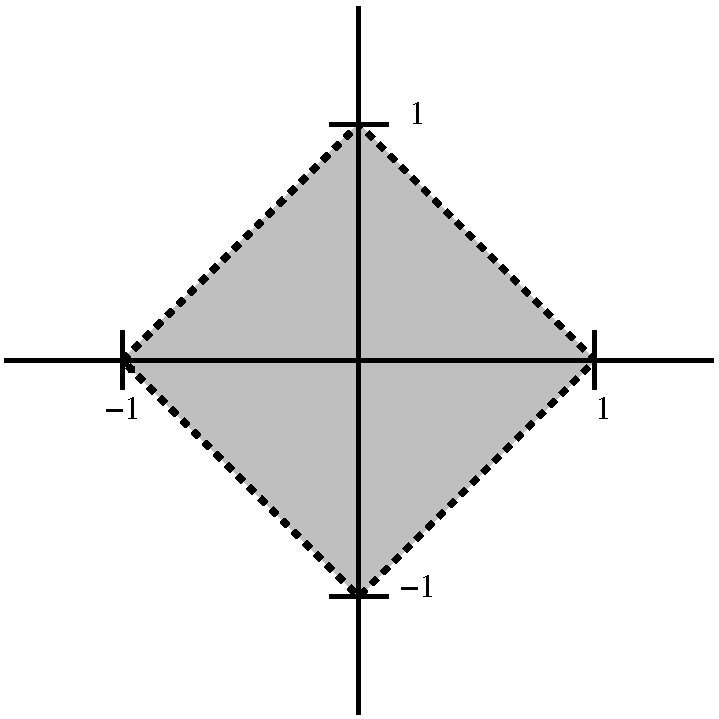
\includegraphics[height=6cm]{figs/ex_20_1_1}
  \end{center}
  Now we show that $d'$ is a metric and induces the usual topology of $\reals^n$.
  \qproof{
    It is easy to see that $d'$ meets the properties required of a metric.
    Clearly $d'(\vx, \vy) \geq 0$ since each $\abs{x_i - y_i} \geq 0$, and $d'(\vx, \vy) = 0$ if and only if each $x_i = y_i$ so that $\vx = \vy$.
    Also it is obvious that $d'(\vx, \vy) = d'(\vy, \vx)$ since each $\abs{x_i - y_i} = \abs{y_i - x_i}$.
    For the triangle inequality we simply have that
    \ali{
      d'(\vx, \vz) &= \sum_{i=1}^n \abs{x_i - z_i} \\
      &\leq \sum_{i=1}^n \parens{\abs{x_i - y_i} + \abs{y_i - z_i}} & \text{(since each $\abs{x_i-z_i} \leq \abs{x_i-y_i} + \abs{y_i-z_i}$)} \\
      &= \sum_{i=1}^n \abs{x_i - y_i} + \sum_{i=1}^n \abs{y_i - z_i} \\
      &= d'(\vx, \vy) + d'(\vy, \vz) \,.
    }

    We now show that the metric topology induced by $d'$ is the same as that induced by the square metric $\r$, which shows the desired result since the square metric induces the standard product topology on $\reals^n$ by Theorem~20.3.
    First consider any $\vx \in \reals^n$ and any $\e > 0$.
    Let $\d = \e$ and consider any $\vy \in B_{d'}(\vx, \d)$.
    Suppose also that $j$ is an index in $\intsfin{n}$ where
    \gath{
      \r(\vx, \vy) = \max\braces{\abs{x_1 - y_1}, \ldots, \abs{x_n - y_n}} = \abs{x_j - y_j} \,.
    }
    Since $\vy \in B_{d'}(\vx, \d)$, we have
    \gath{
      d'(\vx,\vy) = \sum_{i=1}^n \abs{x_i - y_i} < \d = \e \\
      \abs{x_j - y_j} + \sum_{i \neq j} \abs{x_i - y_i} < \e \\
      \abs{x_j - y_j} < \e - \sum_{i \neq j} \abs{x_i - y_i} \leq \e \\
      \r(\vx, \vy) < \e
    }
    since of course $\sum_{i \neq j} \abs{x_i - y_i} \geq 0$.
    Therefore $\vy \in B_\r(\vx,\e)$, which shows $B_{d'}(\vx, \d) \ss B_\r(\vx, \e)$ so that the metric topology of $d'$ is finer the the metric topology of $\r$ by Lemma~20.2.

    Now again consider and $\vx \in \reals^n$ and $\e > 0$, and this time let $\d = \e/n$.
    Consider any $\vy \in B_\r(\vx, \d)$ and again  suppose also that $j$ is an index in $\intsfin{n}$ where
    \gath{
      \r(\vx, \vy) = \max\braces{\abs{x_1 - y_1}, \ldots, \abs{x_n - y_n}} = \abs{x_j - y_j} \,.
    }
    We then have
    \gath{
      \abs{x_j - y_j} = \r(\vx, \vy) < \d = \e/n \\
      n \abs{x_j - y_j} < \e \,.
    }
    We also have
    \ali{
      d'(\vx, \vy) &= \sum_{i=1}^n \abs{x_i - y_i} \\
      &\leq \sum_{i=1}^n \abs{x_j - y_i} & \text{(since each $\abs{x_i - y_i} \leq \abs{x_j - y_j}$)} \\
      &= n \abs{x_j - y_j} \\
      &< \e
    }
    so that $\vy \in B_{d'}(\vx, \e)$.
    Hence $B_\r(\vx, \d) \ss B_{d'}(\vx, \e)$ so that the metric topology of $\r$ is also finer than that of $d'$ again by Lemma~20.2.
    Therefore it must be that the two topologies are equal since each is finer than the other.
  }

  (b) Let $d$ denote the metric defined in part (a), that is
  \gath{
    d(\vx, \vy) = \sum_{i=1}^n \abs{x_i - y_i} \,.
  }
  First we show that the metric topology induced by $d'$ is finer than that induced by $\rho$.
  So consider any $\vx \in \reals^n$ and $\e > 0$.
  Let $\d = \e$ and suppose that $\vy \in B_{d'}(\vx, \d)$ so that
  \gath{
    d'(\vx, \vy) = \parens{\sum_{i=1}^n \abs{x_i - y_i}^p}^{1/p} < \d = \e \,.
  }
  Suppose that $j$ is an index in $\intsfin{n}$ where
  \gath{
    \r(\vx, \vy) = \max\braces{\abs{x_1 - y_1}, \ldots, \abs{x_n - y_n}} = \abs{x_j - y_j} \,.
  }
  Then
  \gath{
    \abs{x_j - y_j}^p \leq \abs{x_j - y_j}^p + \sum_{i \neq j} \abs{x_i - y_i}^p = \sum_{i=1}^n \abs{x_i - y_i}^p
  }
  so that, by Corollary~\ref{cor:metric:opmon}, we have
  \gath{
    \parens{\abs{x_j - y_j}^p}^{1/p} \leq \parens{\sum_{i=1}^n \abs{x_i - y_i}^p}^{1/p} < \e \\
    \abs{x_j - y_j} < \e \\
    \r(\vx, \vy) < \e \,.
  }
  Therefore $\vy \in B_\r(\vx, \e)$ so that $B_{d'}(\vx, \d) \ss B_\r(\vx, \e)$.
  This suffices to show that the metric topology induced by $d'$ is finer than that induced by $\rho$ by Lemma~20.2.

  Now we show that the metric topology induced by $d$ is finer than that induced by $d'$.
  So again consider any $\vx \in \reals^n$ and $\e > 0$.
  Again let $\d = \e$ and suppose that $\vy \in B_d(\vx, \d)$ so that
  \gath{
    d(\vx, \vy) = \sum_{i=1}^n \abs{x_i - y_i} < \d = \e \,.
  }
  Then, since each $\abs{x_i - y_i} \geq 0$, we have by Lemma~\ref{lem:metric:polynom} that
  \ali{
    \sum_{i=1}^n \abs{x_i - y_i}^p &\leq \parens{\sum_{i=1}^n \abs{x_i - y_i}}^p \\
    \parens{\sum_{i=1}^n \abs{x_i - y_i}^p }^{1/p} &\leq \squares{\parens{\sum_{i=1}^n \abs{x_i - y_i}}^p}^{1/p} \\
    d'(\vx, \vy) &\leq \sum_{i=1}^n \abs{x_i - y_i} < \e \,,
  }
  where we have used Corollary~\ref{cor:metric:opmon} in the second step.
  Thus $\vy \in B_{d'}(\vx, \e)$ so that $B_d(\vx, \d) \ss B_{d'}(\vx, \e)$.
  This of course shows that the metric topology induced by $d$ is finer than that induced by $d'$ by Lemma~20.2 again.

  Thus we have shown that the metric topology induced by $d'$ is finer than that induced by $\r$, and also that that induced by $d$ is finer than that induced by $d'$.
  But it was shown in part (a) and Theorem~20.3 that those induced by $d$ and $\r$ are the same topology, which is is the usual product topology on $\reals^n$.
  Hence if $\cT_p$ denotes this usual product topology, we have
  \gath{
    \cT_p = \cT_\r \ss \cT_{d'} \ss \cT_d = \cT_\r = \cT_p \,.
  }
  So it must be that the metric topology induced by $d'$ is this topology as well as desired.
}


\exercise{2}{
  Show that $\reals \times \reals$ in the dictionary order topology is metrizable.
}
\sol{
  \dwhitman

  \qproof{
    In what follows let
    \gath{
      \bd(x,y) = \min\braces{\abs{x-y}, 1}
    }
    be the standard bounded metric on $\reals$, noting that this is a metric by Theorem~20.1.
    Now define the function $d : \reals^2 \times \reals^2 \to \reals$ by
    \gath{
      d(\vx, \vy) = \begin{cases}
        1 & x_1 \neq y_1 \\
        \bd(x_2, y_2) & x_1 = y_1 \,.
      \end{cases}
    }
    We claim that this is a metric on $\reals^2$ that induces the dictionary order topology.

    First we show that $d$ is a metric on $\reals^2$.
    Clearly $d(\vx, \vy) \geq 0$ since both $1 \geq 0$ and $\bd(x_2, y_2) \geq 0$ since $\bd$ is a metric.
    Moreover if $\vx = \vy$ then $x_1 = y_1$ and $x_2 = y_2$ so that $d(\vx, \vy) = \bd(x_2,y_2) = 0$.
    Conversely if $d(\vx, \vy) = 0$ then clearly $d(\vx, \vy) \neq 1$ so that it must be that $x_1 = y_1$ and $d(\vx, \vy) = \bd(x_2,y_2) = 0$ so that $x_2 = y_2$ since $\bd$ is a metric.
    From this it follows that $\vx = \vy$ since $x_1 = y_1$ and $x_2 = y_2$, which shows property (1) of a metric.

    It is also obvious that $d(\vx, \vy) = d(\vy, \vx)$ since if $x_1 \neq y_1$ then $d(\vx,\vy) = 1 = d(\vy, \vx)$.
    If $x_1 = x_2$ then $d(\vx, \vy) = \bd(x_2,y_2) = \bd(y_2,x_2) = d(\vy, \vx)$ since $\bd$ is a metric.
    This shows property (2) of a metric.
    Lastly, consider $\vx$, $\vy$, and $\vz$ in $\reals^2$.

    Case: $x_1 \neq z_1$.
    Then $d(\vx, \vz) = 1$ and it must be that either $y_1 \neq x_1$ or $y_1 \neq z_1$ since otherwise we would have that $x_1 = y_1 = z_1$.
    Thus either $d(\vx, \vy) = 1$ or $d(\vy, \vz) = 1$ and hence
    \gath{
      d(\vx, \vy) + d(\vy, \vz) \geq 1 = d(\vx, \vz)
    }
    since both $d(\vx, \vy) \geq 0$ and $d(\vy, \vz) \geq 0$.

    Case: $x_1 = z_1$.
    Then $d(\vx, \vz) = \bd(x_2,z_2)$.
    If $y_1 = x_1$ then $x_1 = y_1 = z_1$ so that
    \gath{
      d(\vx, \vz) = \bd(x_2,z_2) \leq \bd(x_2,y_2) + \bd(y_2,z_2) = d(\vx,\vy) + d(\vy,\vz)
    }
    since $\bd$ is a metric.
    If $y_1 \neq x_1$ then $y_1 \neq x_1 = z_1$, and hence $d(\vx, \vy) = d(\vy, \vz) = 1$ so that
    \gath{
      d(\vx, \vz) = \bd(x_2, z_2) \leq 1 \leq 2 = 1 + 1 = d(\vx, \vy) + d(\vy, \vz)
    }
    since $\bd$ is the bounded metric so that it is always at most 1.

    Thus in all cases we have shown property (3) of a metric.

    In what follows let $\prec$ denote the dictionary order on $\reals^2$.
    To show that $d$ induces the dictionary order topology, first consider any point $\vx \in \reals^2$ and any basis element $B$ of the dictionary order topology that contains $\vx$.
    Then of course $B = (\va, \vb)$, where $\va \prec \vx \prec \vb$ since the dictionary order has no largest or smallest elements in $\reals^2$.
    Now define
    \gath{
      \d_a = \begin{cases}
        1 & x_2 = a_2 \\
        \abs{x_2 - a_2} & x_2 \neq a_2
      \end{cases}
    }
    and
    \gath{
      \d_b = \begin{cases}
        1 & x_2 = b_2 \\
        \abs{x_2 - b_2} & x_2 \neq b_2 \,,
      \end{cases}
    }
    and let $\d = \min\braces{1, \d_a, \d_b}$.
    Clearly the set $B_d(\vx, \d)$ is a basis element of the topology induced by $d$, and we claim that $\vx \in B_d(\vx, \d) \ss B$.

    That $\vx \in B_d(\vx, \d)$ is obvious.
    So now consider any $\vy \in B_d(\vx, \d)$ so that $d(\vx, \vy) < \d \leq 1$.
    Hence it cannot be that $x_1 \neq y_1$ by definition, since $d(\vx, \vy) = 1$ in that case,  and so $x_1 = y_1$.
    If $x_2 = a_2$ then it has to be that $a_1 < x_1$ since otherwise it would not be the case that $\va \prec \vx$.
    Thus we have $a_1 < x_1 = y_1$ so that $\va \prec \vy$.

    On the other hand if $x_2 \neq a_2$ then it must be that $a_1 \leq y_1$ since otherwise we would have $x_1 = y_1 < a_1$ so that $\vx \prec \va$.
    If $a_1 < y_1 = x_1$ then of course $\va \prec \vy$ so assume that $a_1 = y_1 = x_1$.
    The it must be that $a_2 < x_2$ since $\va \prec \vx$, and so $\abs{x_2 - a_2} = x_2 - a_2$.
    Then, since $x_1 = y_1$, we have that $\bd(x_2, y_2) = d(\vx, \vy) < \d \leq 1$ so it must be that $d(\vx, \vy) = \bd(x_2, y_2) = \abs{x_2 - y_2}$.
    Also $\d_a = \abs{x_2 - a_2} = x_2 - a_2$ since $x_2 \neq a_2$.
    Hence we have $\abs{x_2 - y_2} = d(\vx, \vy) < \d \leq \d_a = x_2 - a_2$, from which it readily follows that $a_2 < y_2$ so that again $\va \prec \vy$.

    Therefore in all cases $\va \prec \vy$.
    Analogous arguments show that $\vy \prec \vb$ so that $\vy \in (\va, \vb) = B$, which shows that $B_d(\vx, \d) \ss B$ as desired since $\vy$ was arbitrary.
    This shows that the topology induced by $d$ is finer than the dictionary order topology by Lemma~13.3.

    Now again suppose that $\vx \in \reals^2$, and that $\e > 0$ so that $B_d(\vx, \e)$ is an arbitrary basis element of the metric topology induced by $d$ that contains $\vx$.
    Let $\d = \min\braces{1, \e}$ and define $\va = x_1 \times (x_2 - \d)$ and $\vb = x_1 \times (x_2 + \d)$.
    Set $B = (\va, \vb)$, which is clearly a basis element of the dictionary order topology.
    So consider any $\vy \in B$ so that $\va \prec \vy \prec \vb$.
    Clearly it must be that $a_1 = y_1 = b_1 = x_1$ since otherwise we would have that $\vy \prec \va$ or $\vb \prec \vy$.
    From this it follows that $a_2 = x_2 - \d < y_2 < x_2 + \d = b_2$ so that $-\d < y_2 - x_2 < \d$ and hence $\abs{x_2 - y_2} < \d$.
    Moreover, since $y_1 = x_1$ and $\d \leq 1$, it follows that $d(\vx, \vy) = \bd(x_2, y_2) = \abs{x_2 - y_2} < \d \leq \e$.
    This shows that $\vy \in B_d(\vx, \e)$, which shows that $B \ss B_d(\vx, \e)$ since $\vy$ was arbitrary.
    This proves that the dictionary order topology is finer than the topology induced by $d$ again by Lemma~13.3.

    Since each is finer than the other the topologies must be the same, which shows that the dictionary order topology is metrizable as desired.
  }
}
